\chapter{Clusters}

Clusters are aggregations of atoms or molecules connected via non-covalent
bonds such as van der Waals forces, hydrogen bonds or metallic bonding.
They are an interesting
matter because their properties lie in between the properties of on the one hand
atoms and molecules and solid state matter on the other hand.

The investigation of clusters touches the basic question, from what point
on a solid actually is a solid matter and not a very big cluster.
Very often this question is answered by the number of constituents
of a cluster being
2 -- 50000, but from an other point of view, the decision for
a system to be a cluster or a solid can be drawn by looking for
intrinsic 
properties of solids in the system under investigation.
Nevertheless, not all criteria might allow to draw the same conclusion.
%This question can be answered looking at several property criteria of solids,
%but the criteria not necessarily allow to draw the same conclusion.

In solids atoms or molecules ideally have a fixed postion with respect to their
neighbours. These structures can be very ordered like in crystals and metals
or amorphous. In all cases the microscopic structure is characterizing for
the material and also determines its macroscopic
porperties.
The structures can differ between small clusters and the macroscopic
material. For example small rare gas clusters show an overall icosahedral
structure, whereas the solid shows a space filling fcc structure with
a distinct bondlength between every atom with its nearest neighbours.
A transition of the most favourable strucutre pattern can be utilized
for the transition between a cluster and the solid.

Solids are able to both melt and sublimate. Microscopically melting
is being defined as atoms or
molecules changing from having a fixed position within the ensemble to a
random position with respect to their neighbours, but still being part
of the clusters, whereas sublimation can be defined as atoms or molecules
moving far enough away from the rest of the cluster to not being captured
again.
Both melting and sublimation themselves can be achieved already for very
small clusters
sizes consisting of not more than two atoms. From a certain size on,
clusters melt and sublimate under the same conditions as macroscopic
solids.

Further criteria can be conductivity and magnetic susceptibility.

Research on clusters very often use noble gas clusters as workhorses for
the investigation of basic properties.
In general atoms are preferred for the investigation of clusters because
they are spherical symmetric and hence the orientation of the substituents
in the cluster is not to be investigated.
Noble gases as such are theoretically easy to describe because of their
electronic closed shell structure.
They only interact via
van der Waals forces and hence the atomic electronic states are very
localized to a specific atom and are therefore
reasonably well starting points for the description of atoms within the
clusters. 
Additionally the electronic closed shell structure leads to a very well
defined ground states which allows to neglect difficulties arising from
multi-reference states.

Experimentally rare gases clusters are beneficial because the noble gases
already are gaseous, are
thermically stable, easy to introduce into the apparatus
and the cleaning of the
apparatus after the experiment is fast and easily done compared to
e.g. metals.


\section{Noble Gas Clusters}
Noble gas clusters contain noble gases of either one or several types of
noble gas atoms. The several atoms can be classified based on
their position within a cluster. Atoms in the bulk are surrounded by
neighbours, whereas atoms in the surface region miss interaction
partners on at least on side as displayed in figure \ref{figure:cluster_cut} showing
a cut through a cuboctahedral cluster.

\begin{figure}[h]
 \centering
 \begin{minipage}[htb]{0.4\textwidth}
   \centering
   \begin{tikzpicture}[scale=1.0,>=stealth]
       %\tiny
       %\draw [help lines] (-3,-3) grid (5,5);
       \draw [diplom1,pattern color=diplom1,pattern=north east lines,thick]
             (0:0) circle (0.5);
       \foreach \alpha in {0,60,...,300}
         \draw [diplom1,pattern color=diplom1,pattern=north east lines,thick]
               (\alpha : 1.0) circle (0.5);
       \foreach \alpha in {0,60,...,300}
         \draw [diplom2,pattern color=diplom2,pattern=north east lines,thick]
               (\alpha : 2.0) circle (0.5);
       \foreach \alpha in {30,90,...,330}
         \draw [diplom2,pattern color=diplom2,pattern=crosshatch,thick]
               (\alpha : 1.7321) circle (0.5);
   \end{tikzpicture}
\end{minipage}
\hspace{0.5cm}
\begin{minipage}[htb]{0.4\textwidth}
%Legende
\addlegendimageintext{pattern=north east lines, pattern color=diplom1, area legend} core atom

\addlegendimageintext{pattern=north east lines, pattern color=diplom2, area legend} surface atom -- vertex

\addlegendimageintext{pattern=crosshatch, pattern color=diplom2, area legend} surface atom -- edge
\end{minipage}

 \caption{Cut through a cuboctahedral cluster illustrating the different
          kinds of atoms within a cluster. The bright blue colored atoms
          are bulk atoms whereas the dark blue atoms belong to the surface.
          Within a shell atoms can either be vertices (striped), belong to
          an edge (crosshatched) or lie within a layer (not depicted in this
          two dimensional sketch.}
 \label{figure:cluster_cut}
\end{figure}

Within a shell each atom either is a vertex atom, an atom in an edge
or in plane as shown in figure \ref{figure:cluster_cut}.

The noble clusters are held together by the London dispersion force
stemming from the interaction of induced dipole moments in the polarizable
noble gas atoms, which is a special case of the van der Waals forces.
The interaction potential between two atoms is therefore reasonably
well described by the so called
Lennard-Jones potential

\begin{equation}
  V_{LJ}(R) = 4 \varepsilon \left( \left(\frac{\sigma}{R}\right) ^{12}
              - \left(\frac{\sigma}{R}\right) ^{6} \right)
\end{equation}
where R denotes the internuclear distance, 
and $\varepsilon$ is the depth of the
potential. Due to different conventions of the formulation
of the Lennard-Jones potential $\sigma=\frac{R_{min}}{\sqrt[6]{2}}$
with $R_{min}$ being the distance of the potential minimum.

\begin{figure}[h]
 \centering
 \begin{tikzpicture}
    \begin{axis}[domain=3.2:9.0,
                 samples = 200,
                 xtick={3,5,...,9},
                 %xticklabels={$-\pi$,$-\frac \pi 2$,0,$\frac \pi 2$,$\pi$},
                 extra x ticks={3.82086},
                 extra x tick labels={$\sqrt[6]{2} \sigma$},
                 cycle list name = exotic,
%                 legend style={anchor= north west},
                 xlabel = {R [\AA]},
                 ylabel = {V [meV]}
                 ]
    \addplot+[mark = none,
             thick,
             diplom1
             ]
             {4*12.4 * ( (3.404/x)^(12) -  (3.404/x)^(6) )}; 
    \addlegendentry{Ar-Ar}
    \addplot+[mark = none,
             dashed,
             gray
             ]
             {0.0}; 
    \addplot+[mark = none,
             dashed,
             gray
             ]
             {-12.4}; 
    \draw [thick,<->] (axis cs:8.0,-12.4) --
          node [right=2pt] {$\varepsilon$} (axis cs:8.0,0.0);
    
    \end{axis}
\end{tikzpicture}

 \caption{Lennard-Jones potential of the argon dimer illustrating the
          Lennard-Jones parameters $\sigma$ and $\varepsilon$.}
 \label{figure:LJ_Ar2}
\end{figure}

It contains a repulsiv part, taking care of the description of the
Pauli repulsion due to overlapping orbitals at short distances. The
$R^{-12}$ dependency is not theoretically justified but convenient
for an analytic description. The attractive $R^{-6}$ part describes
the London dispersion interaction.
For the different noble gases the Lennard-Jones parameters are given in
table \ref{table:LJ_parameter} and the potentials are shown in
figure \ref{figure:LJ_Ar2}.

\begin{table}[htb]
 \caption{Lennard-Jones parameters for noble gas dimers used in this
          thesis.}
 \centering
 \begin{tabular}{lcc}
   \toprule
   Atom type & $\sigma$ [\unit{\AA}] & $\varepsilon$ [\unit{meV}]\\
   \midrule
   Ne-Ne     & &\\
   Ne-Ar     &&\\
   Ar-Ar     &                 3.404 & 12.4\\
   Ar-Xe     &                 3.72  & 14.4\\
   Xe-Xe     &                 3.961 & 23.1\\
   \bottomrule
 \end{tabular}
 \label{table:LJ_parameter}
\end{table}


Homonuclear noble gas clusters from the distance look like a sphere
because for minimizing
the energy of the cluster the interaction between them needs to be
maximized. Atoms at the surface of a cluster have less interaction
partners than atoms in the bulk and the three dimensional structure
with the smalles surface to volume
ratio $\frac{S}{B}$ is the sphere. 

At a closer look the structure is not able to be a perfect sphere
because of the shape of the constituing atoms. Both theoretical
calculations and mass spectrometry of rare gas mixtures show, that
for small clusters, the icosahedral structure, where icosahedral
shells are nested into each other, is energetically beneficial.
For a more detailed description on how to construct such an icosahedral
structure see \ref{}.

The number of atoms can be calculated via

\begin{equation}
  n_{atoms} = \frac{10}{3} c^3 - 5 c^2 + \frac{11}{3} c -1 .
\end{equation}

where $x$ denotes the number of shells, where the central atom is
also counted as a shell. \cite{Martin96} This way, $c$ is
identical to the number of atoms
in the edge of the outermost shell.


In contrast to this, larger clusters and the solid show a cuboctahedral
pattern, which infinitely extended leads to a \ac{fcc} structure.
In the \ac{fcc} structure every atom is symmetrically surrounded
by 12 atoms in the same distance, while in icosahedral structures, the
atomic distance between atoms of different shells are smaller than the
interatomic distance within a shell. A large number of surface atoms
will therefore induce an icosahedral structure.
The larger the clusters are, the smaller is their surface to bulk
ratio $\frac{S}{B}$ and therefore the influence of of the surface
atoms on the overall structure decreases as illustrated in
figure \ref{figure:surface_to_bulk}. From a certain size on the
preferred structure changes from icosahedral to cuboctahedral. This size
is not exactly known and a topic of ongoing research. It is well accepted,
that the transition is supposed to lie somewhere between \unit[800--3000]{atoms},
which corresponds to $c = 7 - 11$.

\begin{figure}[h]
 \centering
 \begin{tikzpicture}
    \begin{axis}[domain=2.0:13,
                 samples = 12,
                 %xtick={3,5,...,9},
                 %xticklabels={$-\pi$,$-\frac \pi 2$,0,$\frac \pi 2$,$\pi$},
                 %extra x ticks={3.82086},
                 %extra x tick labels={$\sqrt[6]{2} \sigma$},
                 cycle list name = exotic,
%                 legend style={anchor= north west},
                 ylabel = {$\frac{{surface}}{{bulk}}$},
                 xlabel = {$c$}
                 ]
    \addplot[mark = *,
             thick,
             diplom1
             ]
             {(10/3*x^3 - 5*x^2 + 11/3*x -1) /
              (10/3*(x-1)^3 - 5*(x-1)^2 + 11/3*(x-1) - 1) - 1}; 
             %{(10/3*(x-1)^3 - 5*(x-1)^2 + 11/3*(x-1) -1) /
             % ((10/3*x^3 - 5*x^2 + 11/3*x -1) - (10/3*(x-1)^3 - 5*(x-1)^2 + 11/3*(x-1) - 1))}; 
    \end{axis}
\end{tikzpicture}

 \caption{Surface to bulk ratio for icosahedral structures with $c$ complete
          shells illustrating the decreasing impact of the surface atoms.}
 \label{figure:surface_to_bulk}
\end{figure}

The structure of heteronuclear clusters is expected to be similar to the
homonuclear rare gas cluster with a core consisting of the more polarizable
atom type somehow surrounded by atoms of the other atom type, which will be discussed
in the next section. To my knowledge no more detailed information about
the structure of heteronuclear rare gas cluster is known in the
literature. A new method for the investigation of the structure is found
in this thesis.


\section{Creation of Noble Gas Clusters}
In order to create stable clusters, its kinetic energy $k_BT$ needs to be lower
than the sum over the cohesive enrgies in the cluster.
In the experiment, noble gas clusters are formed via expansion through
a supersonic jet. The gas flows through the jet, driven by the lower pressure
on the other end of the chamber. If the mean free path of an atom or molecule
$\lambda$ is large compared to the diameter $d$ of the nozzle, then the flow is
molecular. In case of $\lambda$ being much smaller than $d$, the atoms inside
the nozzle collide and thereby unify their velocity to the group velocity
in direction of the stream. Consequently the width of the lateral velocity
distribution is decreased and due to energy conservation the temperature
in expansion direction is decreased, which allows the formation of clusters.
When all atoms have the same velocity, the atoms do not collide any longer
and hence, sound would not be transferred through this medium. Therefore,
such a stream of atoms or molecules is called a supersonic jet.

Cluster growth starts with the creation of a dimer. Due to energy conservation
a three-particle collision is required. Two particles form a dimer and the
third particle removes kinetic energy. For all further additions of particles
a two particle collision is sufficient. The kinetic energy of the additional
atom is then used to excite vibrations within the cluster.

The likelihood for three-particle collisions is proportional to the pressure
in the nozzle squared. By increasing the pressure, therefore the creation
of Kristallisationskeime is supported. On the other hand the apparatus
is limited to the efficiency of the vacuum pump.

Whenever one speaks of rare gas clusters, one has to keep in mind, that
with today's experimental knowledge and apparatus single clusters
inhibiting a defined number of atoms or even structure can not be created.
In every experiment a whole manifold of clusters with different sizes are
formed. This manifold is characterized by the average number of atoms
per cluster $\bar{N}$. This number is not necessarily the most probable
cluster in the mixture as can easily be seen from figure \ref{figure:}.
The width of the cluster size distribution is normally estimated to be
$2\bar{N}$.

\begin{figure}[h]
  \centering
%figure with size distribution
  \caption{}
  \label{}
\end{figure}

The mean cluster size $\bar{N}$ can be estimated with
the help of the empirial scaling parameter $\Gamma^*$ of Hagena et al.
\cite{Hagena} for different experimental conditions.

\begin{equation}
 \Gamma^* = \frac{p_0 d_{eq}^q}{T_0^{5/2-q/4}} K_{ch}
\end{equation}
Here, $p_0$ and $T_0$ are the expansion pressure and the temperature
of the nozzle and $d_{eq}$ is the equivalent nozzle diameter for conical
nozzles. $K_{ch}$ is a constant depending on the material and can be
calculated by the means of \cite{xyz}. The values for the rare gases for
the experimental setup, which will be compared to in this work are
$K_ch(Ne)=185$, $K_ch(Ar)=1646$, $K_ch(Kr)=2980$ and $K_ch(Xe)=5554$.

From the scaling parameter the mean cluster size $\bar{N}$ 
of homonuclear clusters can be
estimated as

\begin{equation}
  \bar{N} = 33 \left( \frac{\Gamma^*}{1000} \right) ^{2.35} .
\end{equation}


\subsection{Creation of Heteronuclear Noble Gas Clusters}
Heteronuclear noble gas clusters can either be created in two different ways:
the \emph{pick-up} method or co-expansion of the two different gases.
For the pick-up method the jet of homonuclear clusters is directed through
a volume with a high concentration of the other species. The clusters
collide with the second species which consequently is attached to the surface
of the parent cluster. Depending on the types of the species
and the experimental conditions only few atoms
of the second species stay on the surface of the parent cluster,
several atoms form a shell around the parent cluster or the second species
diffuses into the bulk of the parent cluster.

In the co-expansion method two gases are mixed before the expansion and
then led into the nozzle together. The species with the higher cohesive
energy is more likely to form dimers which then serve as Kristallkeim of
the cluster growth.



\section{Experimental Analysis Tools}
Noble gas clusters are investigated using mass spectrometry and spectroscopy.
From the mass spectrometry information about the mean number of atoms
can be obtained. Within spectrometry two ansatzes are used
to gain information about clusters. In the first one, measurements of
atomic properties for atoms in clusters are compared to the results of
atoms. From the number of peaks, the energy shift and the relative peak
intensity conclusions about the surroundings about the atoms inside
the cluster are drawn. These methods are \ac{PES}, especially \ac{XPS}
and \ac{UPS}, \ac{AES}, \ac{RAS}, \ac{XES}, \ac{NEXAFS} and \ac{XAS}.
Their different working principles are illustrated in figure
\ref{figure:overview_spectroscopies}.

\begin{figure}[h]
  \centering
  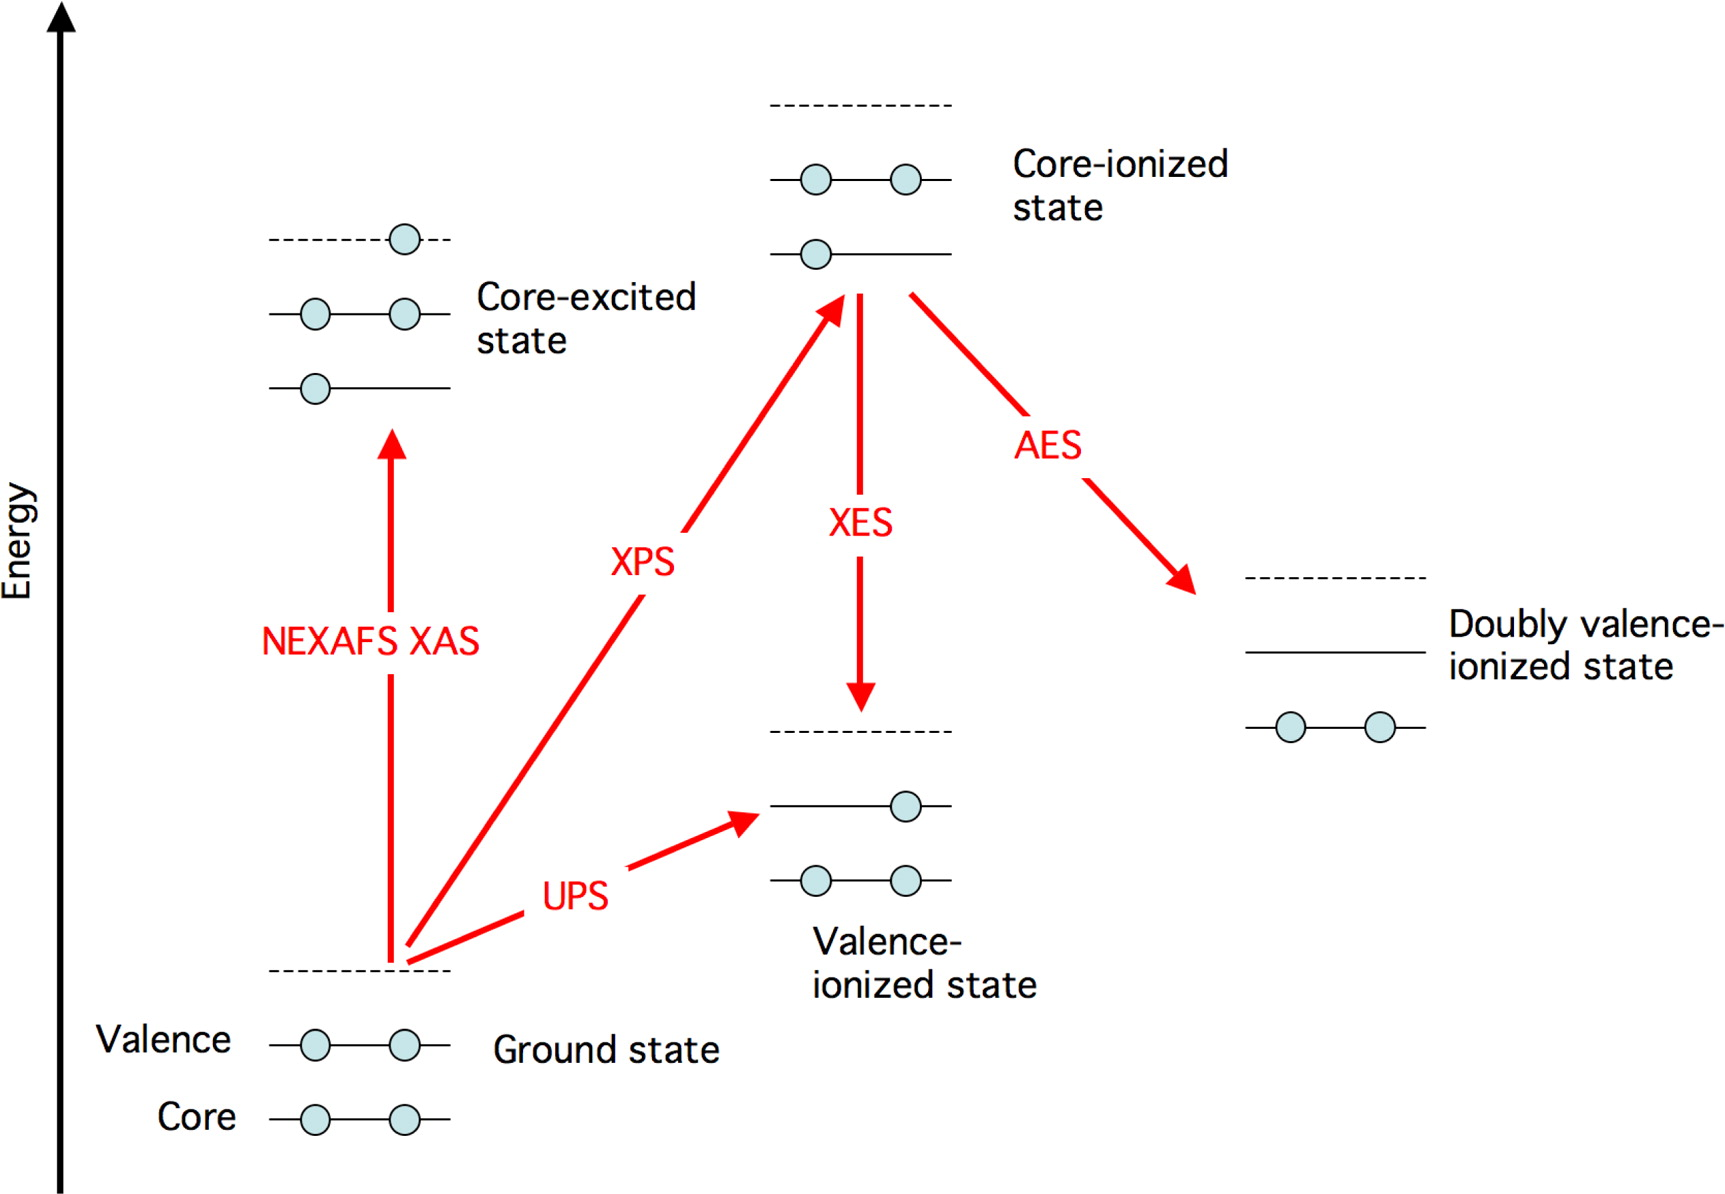
\includegraphics[scale=1.0]{pics/overview_spectroscopies.jpeg}
  \caption{Elsevier Schematic overview over the physical mechanisms of different
           spectroscopic methods.}
  \label{figure:overview_spectroscopies}
\end{figure}

\ac{XAS}, also known as \ac{NEXAFS} probe the absorption of light
from the ground state to a core excited state With \ac{PES} ionization
energies can be determined. More acurately \ac{UPS} gives information
about the ionization potentials of valence orbitals and \ac{XPS}
of core orbitals.
\ac{AES} measures the kinetic energy of the emitted Auger electron
resulting in a doubly (mostly valence) ionized final state, while
\ac{XES} measures the photon emitted during an relaxation from
a core ionized to valence ionized state.

Using thoses techniques atoms in the bulk can be differenciated from atoms
in the bulk and even different positions in the
outermost shell could be resolved. The obtained surface-to-bulk ratios
can then also be used for an estimation of the mean cluster size.

The second ansatz, which is developed in this thesis, uses electron-electron
and ion-ion coincidence spectroscopy.
They exploit the interaction between neighbouring atoms
directly using the ICD.
Until now, these techniques
have been used for the investigation of the
\ac{ICD}, but since the ICD strongly depends on the geometry, I am going to
, that having information about the ICD, conclusions about
the cluster structure can be drawn with the help of experimental
electron-electron spectra.

\begin{figure}[h]
  \centering
  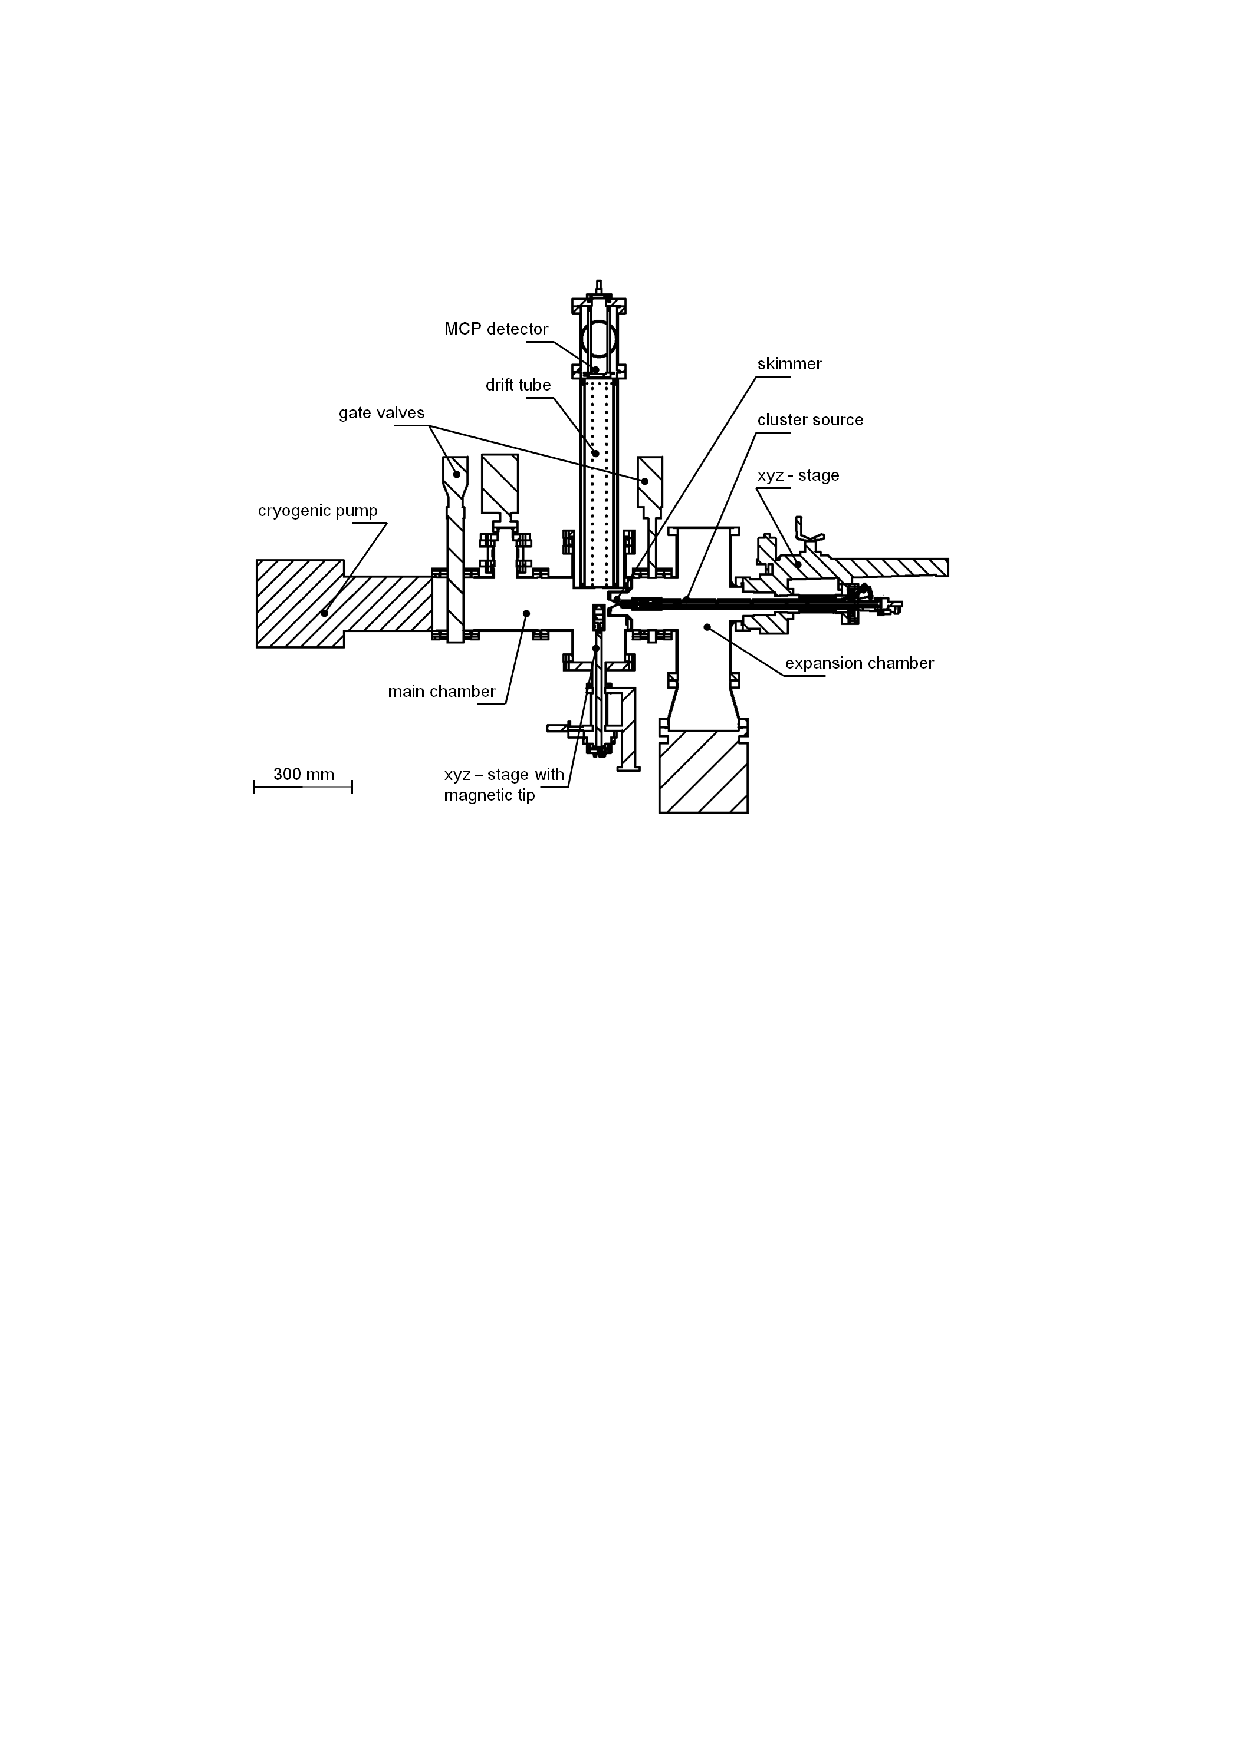
\includegraphics[]{pics/exp_setup_overview.pdf}
  \caption{Schematic view of the experimental setup of a electron-electron
           coincidence measurement. The synchrotron radiation axis
           is perpendicular to the plane of the diagram.}
  \label{figure:exp_setup_overview}
\end{figure}

The principle experimental setup for both coincidence measurements is very similar.
As shown in figure \ref{figure:exp_setup_overview},
the clusters are created using a supersonic jet
and lead through the xyz chamber. Here, perpendicular to the expansion direction
synchrotron radiation enters the reaction chamber with a time of
\unit[]{} between two pulses.
One synchrotron pulse corresponds to one photon, which can be used for the
ionization
of one of the clusters in the stream. The created vacancy can then decay via ICD.
In this case, a second electron is emitted and the two positively charged
subsystems undergo
Coulomb explosion within a timescale of \unit{fs} to \unit[]{ps}.
In this time scale, the ionized cluster is still inside the reaction are sphere.
Initiated by the synchrotron photon four charged particles are created,
two electrons and two ions.
Being charged, these particles can easily be withdrawn from the reaction
chamber to detectors using a so-called magnetic bottle for both positively
and negatively charged particles. In experiments normally only either electrons
or ions are investigated at a time.

A coincidence of two particles is experimentally defined by two events
measured in a specific time range after one synchrotron pulse.
In case of the ion-ion coincidence, this property is called \ac{KER}.
For the
electron-electron coincidence, the coincidence time range is \unit[xyz]{fs}.
Coincidences are very often displayed in a so-called coincidence map,
where the kinetic energy of one electron is plotted against the
kinetic energy of the other electron. 
Two electrons measured in coincidence can stem from several physical
processes. In the coincidence map these processes are distiguishable
from the form of the signal.

\begin{figure}[h]
  \centering
  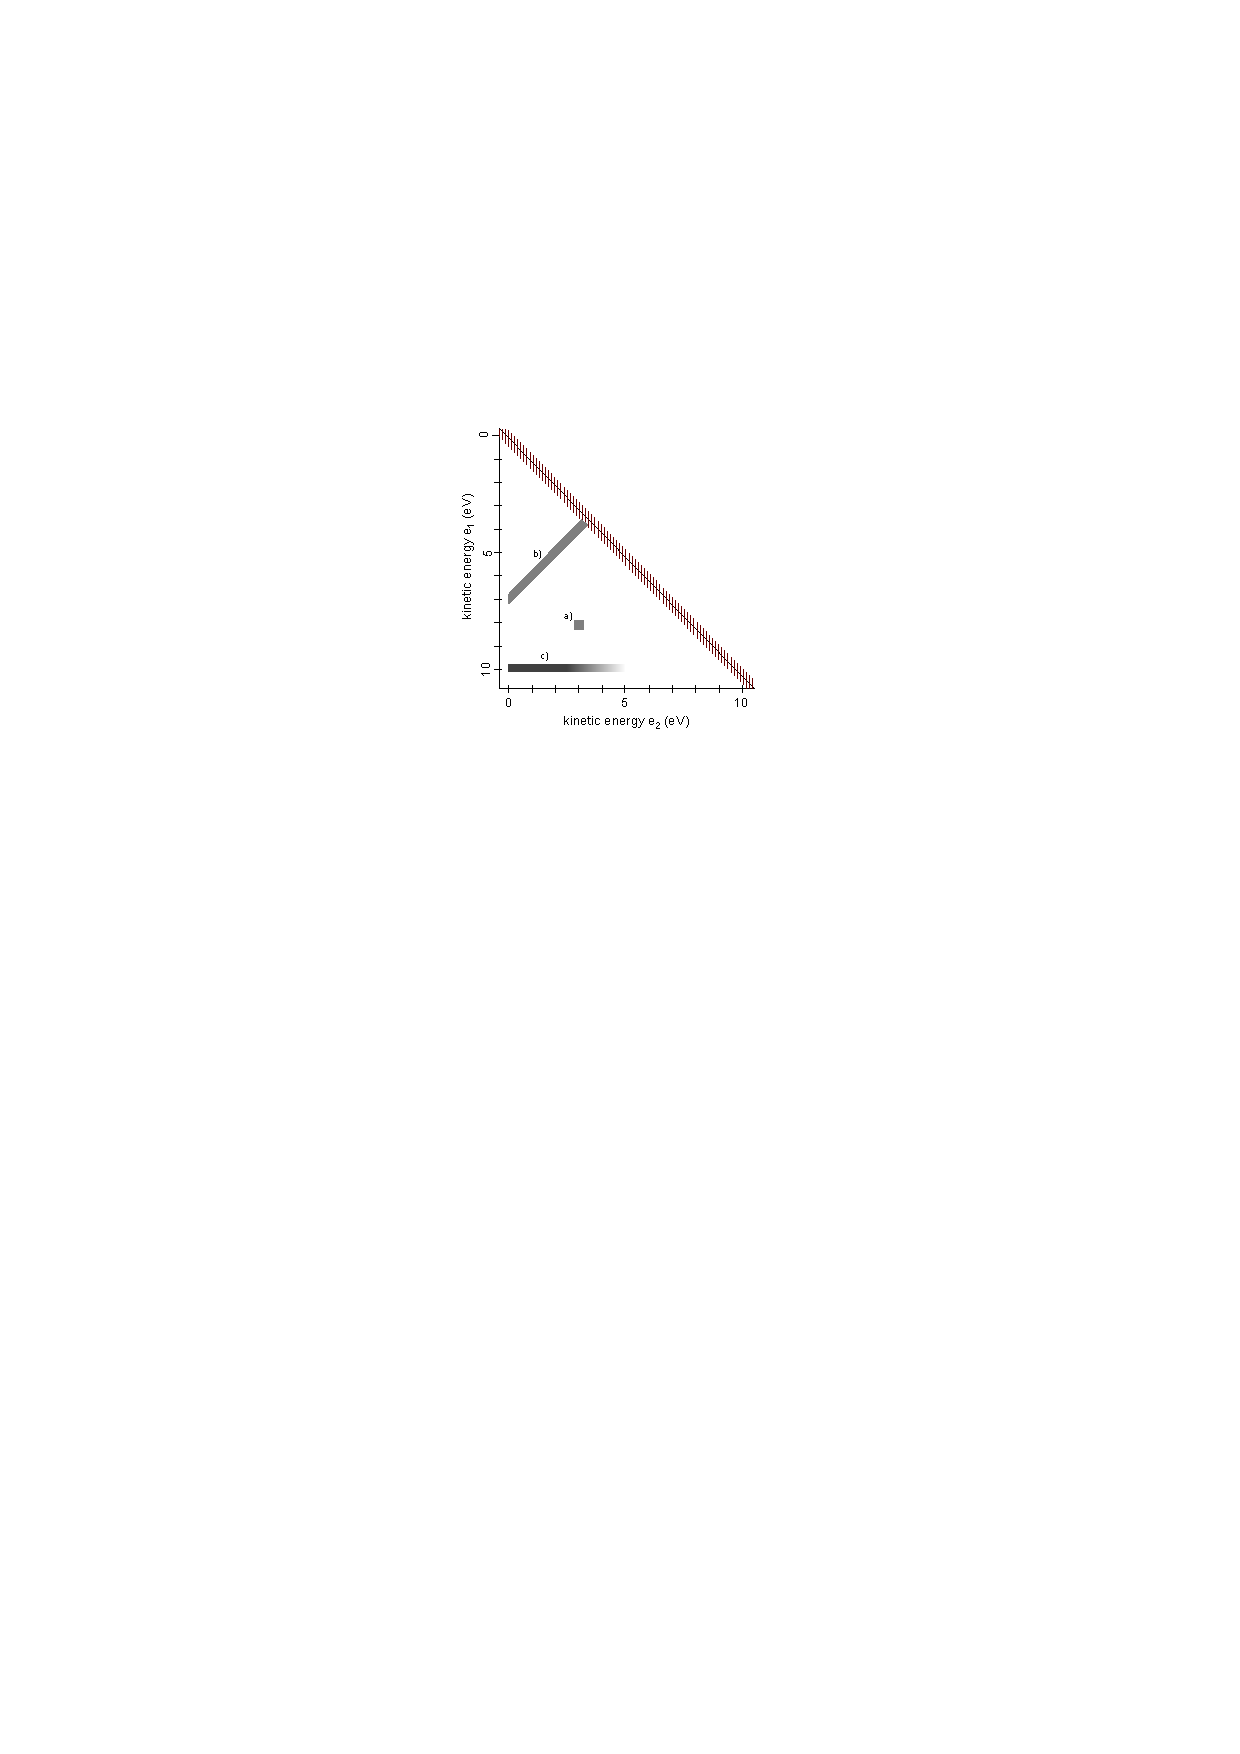
\includegraphics{pics/ee_coincidence_processes.pdf}
  \caption{}
  \label{figure:ee_coincidence_processes}
\end{figure}

Figure \ref{figure:ee_coincidence_processes} illustrates such a coincidence
map. There, the signal a) is a spot at defined energies $e_1$ and $e_2$.
It corresponds to a process, where the electrons both stem from orbitals
of a well defined, small energy range and the final state energy is not
influenced by perturbations like vibrations. This could e.g. be an Auger
decay.
Signal b) is a straight line with a constant sum of the kinetic electron
energies. For example electron-electron scattering shows such a behaviour.
Signal c) is a smeared out line, where one electron energy is constant
and the kinetic energy of the second electron underlies a distribution.
An ICD process would exhibit such a signal. Here the ionization energy
for the creation of the initial state is quite well defined, whereas
the energy of the final states shows a broad distribution due to
vibrations and, as is to be shown in this thesis, due to several decay
channels with different final state energies as well as a decay involving
atoms at different distances inside larger clusters.

For an investigation of an ICD, the experimental data is extracted,
where one of the
electrons is inside the energy range of the kinetic energy
corresponding to the ionization out of
the initial state of interest. The number of counts is then plotted
against the kinetic energy of the second electron to give the ICD electron
spectrum. An example for such a spectrum is shown in
figure \ref{figure:ICD_spectrum_example}


\begin{figure}[h]
  \centering
%  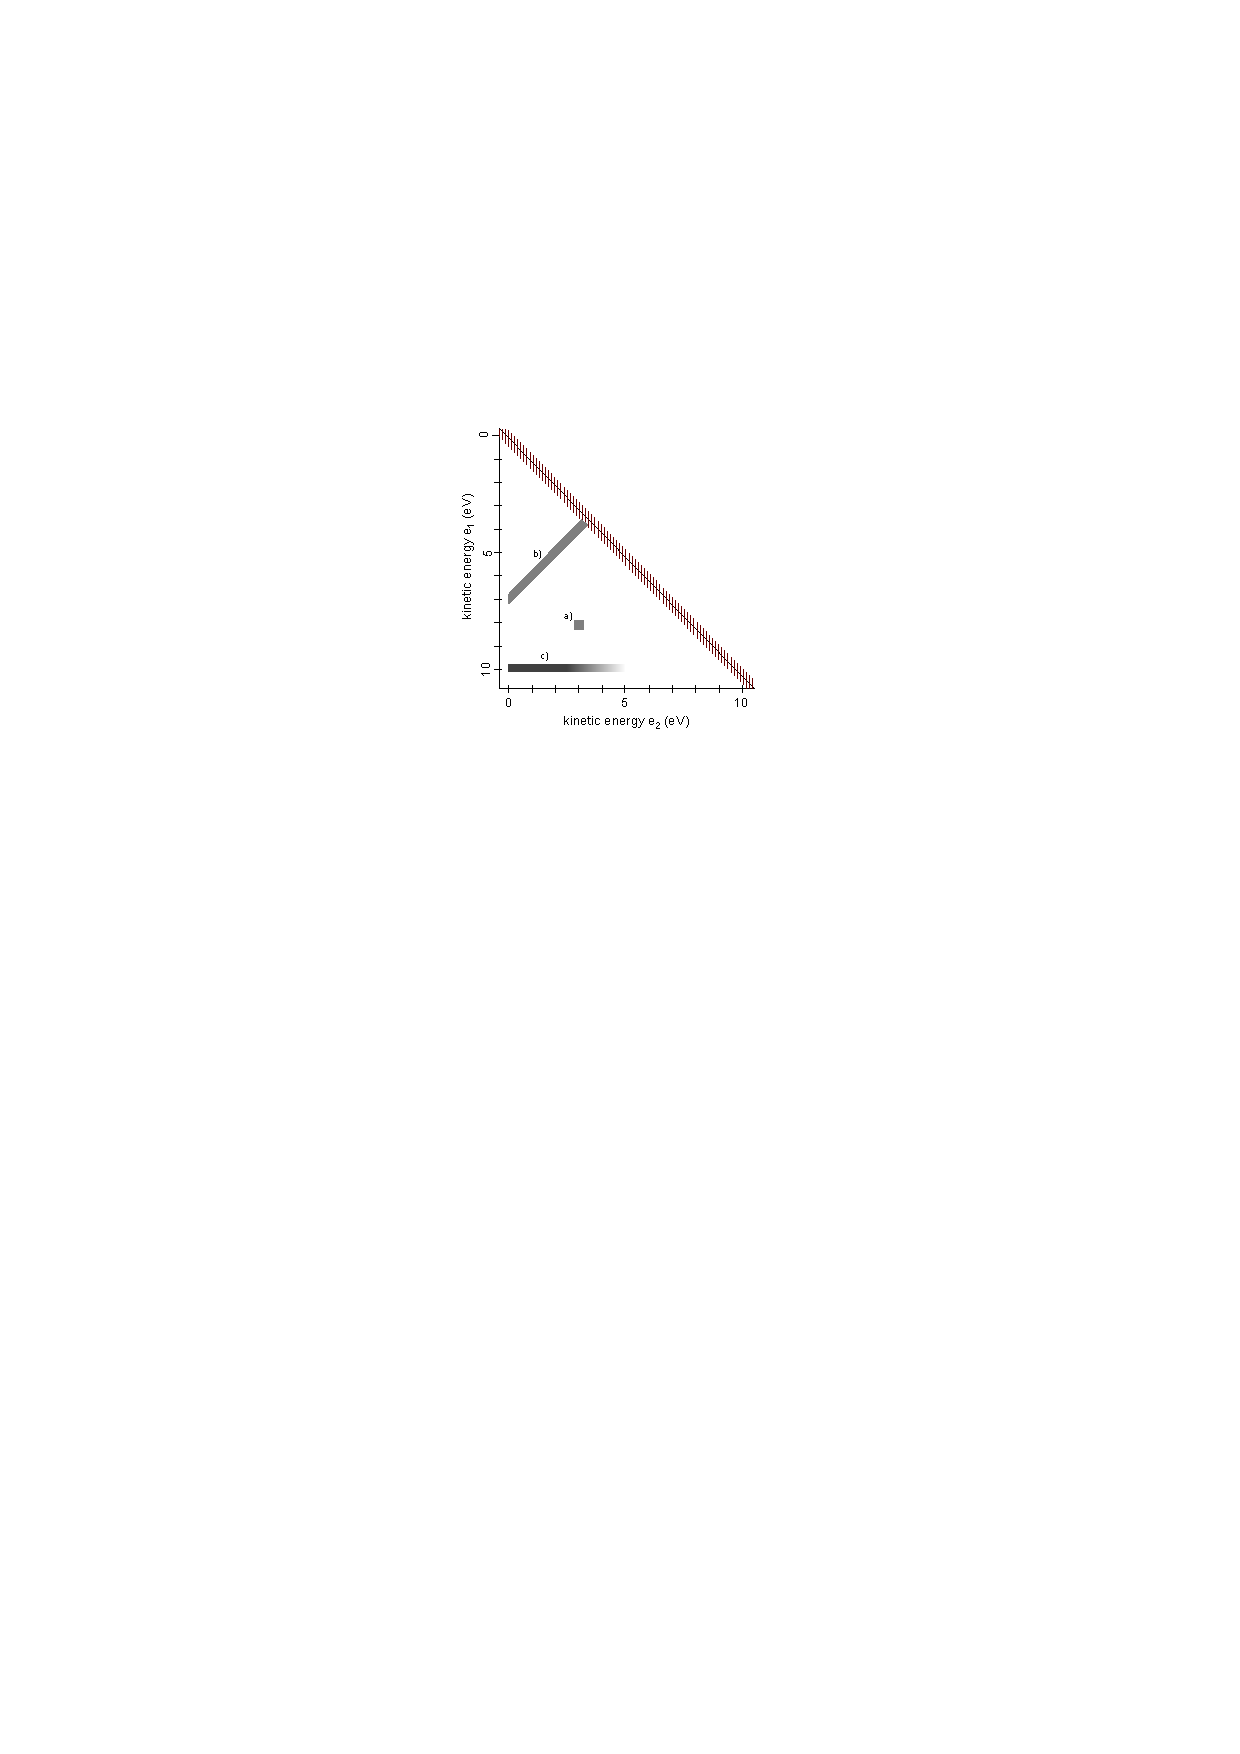
\includegraphics{pics/ee_coincidence_processes.pdf}
  \caption{}
  \label{figure:ICD_spectrum_example}
\end{figure}
